\subsection{Using {\protege} for ontology development}
\label{ssec:using-protege}

{\protege} supports a wide range of features that are useful for various parts of ontology development but going into detail about them is beyond the scope of this guide. This section will only cover a simple description, for a more in-depth introduction, the "New Prot{\'e}g{\'e} Pizza Tutorial"\footnote{\url{https://www.michaeldebellis.com/post/new-protege-pizza-tutorial}} by Michael DeBellis can be a good starting point.


\subsubsection{Enabling alphanumeric identifiers}
By default, {\protege} uses the user supplied name as the identifier of a newly created entity (class, property or individual).

The proposed ontology workflow uses alphanumeric identifiers due to them having multiple advantages e.g. being robust against future entity name changes. These numerical identifiers encode two pieces of information: A unique id for the given entity and the developer that added this entity.

% Alphanumeric identifiers are listed as best practice and commonly used because in most cases their advantages outweigh the disadvantages. A short summary is given below:
% \paragraph{Advantages} 
% \begin{itemize}
%     \item Versioning and backward compatibility: A name for a concept
%     can change in a new version of the ontology without its identifier (in
%     databases etc.) having to be changed everywhere. 
%     \item User groups: If people
%     talk about the same concept but can't decide on a main name for it, they
%     can both be added as labels for this concept and the people can get
%     their own views of the ontology showing their preferred label. 
%     \item Better readability: In labels, we do not have to use CamelCase. Long names like NonRenewableMunicipalWasteFuel are better readable in lower case as ``non renewable municipial waste fuel''.
% \end{itemize}

% \hypertarget{disadvantages}{%
% \paragraph{Disadvantages}\label{disadvantages}}
% \begin{itemize}
% \item
%   The file is harder to read without a tool like Prot\'eg\'e (that will
%   automatically show labels instead of the alphanumerical identifiers).
% \end{itemize}

\paragraph{How to change your settings}\label{how-to-change-your-settings}
{\protege} is able to generate these IRIs automatically, but the required settings are not entirely intuitive. Navigate to \textit{$\text{File}\rightarrow\text{Preferences...}\rightarrow\text{New entities}$} and change the following settings:

\begin{itemize}
    \item \texttt{Entity\ IRI:}
    \begin{itemize}
        \item \texttt{Start with:} Select the \texttt{Specified\ IRI} option and change it to the "Ontology IRI" of your ontology. 
        \item \texttt{Followed by:} This setting depends on how the IRIs are resolved but \texttt{/} is a valid option.
        \item \texttt{End with:} Select the \texttt{Auto-generated\ ID} option.
    \end{itemize}

\item \texttt{Entity Label:} Choose the \texttt{Same as label renderer} option so {\protege} will display the annotated names of entities rather than their identifier in the graphical interface.

\item \texttt{Auto-generated ID:} Choose the \texttt{Numeric (iterative)} option and set the following parameters:
\begin{itemize}
    \item \texttt{Prefix:} [Ontology]\_{[}your user id{]} e.g. MNO\_0001 if your user ID is 1.
    \begin{itemize}
        \item The list of user IDs should be documented in the main ontology file e.g. using the \emph{dc:contributor} annotation. New developers can then add themself via a pull request.
    \end{itemize}
    \item \texttt{Digit count:} The number of digits that your entity identifiers should have, e.g. 4 to allow every user to create 10000 entities before having to get a new ID.
    \item \texttt{Start:} The smallest value for entity identifiers, usually 0.
    \item \texttt{End:} The largest possible value for entity identifiers, usually -1 to disable a maximum value.
\end{itemize}
\end{itemize}
An example for these settings is shown in Figure~\ref{fig:protege-settings}.

\begin{figure}
    \centering
    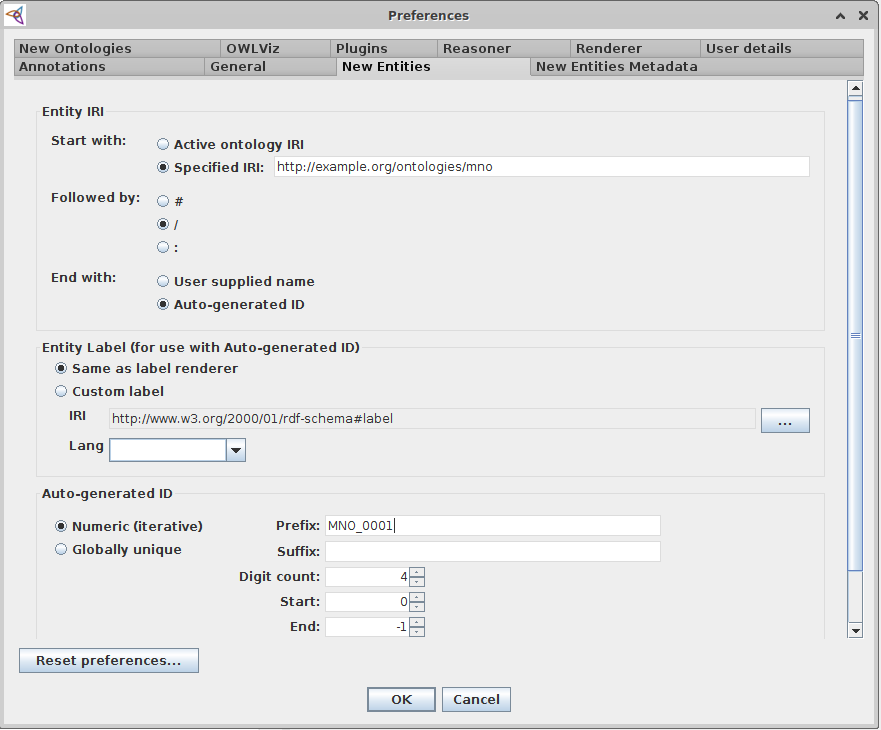
\includegraphics[width=\textwidth]{fig/protege-settings.png}
    \caption{Settings in \textit{$\text{File}\rightarrow\text{Preferences...}\rightarrow\text{New entities}$} as described in Section \ref{how-to-change-your-settings}.}
    \label{fig:protege-settings}
\end{figure}


\subsubsection{Creating a new class}
To create a new class in {\protege}, navigate to the \textit{$\text{Classes}$} tab in the \textit{$\text{Entities}$} tab. Select the class you want to create a subclass from with \texttt{owl:Thing} being the class containing everything. Either use the \textit{Add subclass} button above the hierarchical view or right-click the class and select the \textit{Add subclass...} option. A new window will open where you can enter the name of the class. The IRI of the class will be generated automatically based on the settings described in the previous section. The name will be used for the label annotation of the class and should be displayed to you by {\protege} if the settings are correctly set according to \ref{how-to-change-your-settings}.


\subsubsection{Adding a new axiom}
To add a new axiom to a class, navigate to the \textit{$\text{Classes}$} tab in the \textit{$\text{Entities}$} tab and select the class you want to add the axiom to. On the right side, a tab with the class details - the annotation view on top and the description view below - will open. In the description view, you can see various types of axioms that can be added to the class. By selecting the \textit{+} button next to them, a window will open with various views to construct the axiom you want to add, e.g. \textit{Class hierarchy} to select one of the created classes for the axiom like \texttt{Car}, \textit{Object restriction creator} for restrictions on object properties like \texttt{'has part' exactly 1 'Motor'} or \textit{Class expression editor} for writing those assertions yourself.


\subsubsection{Using the reasoner}
A reasoner is a tool that can be used to infer new knowledge from the axioms in an ontology, e.g. if two properties are inverses of one another, only one axiom needs to be asserted by the user while the reasoner will infer the other. (Inferred knowledge is distinguishable due to it being displayed on a yellow background.)
In Figure~\ref{fig:protege-asserted-class-hierarchy} and Figure~\ref{fig:protege-inferred-class-hierarchy}, the class hierarchy is shown as asserted by the user and as inferred by the reasoner. Both views can be toggled using the dropdown menu in the top right corner of the class hierarchy tab.

The reasoner also serves a different purpose by being able to check whether the ontology is consistent, i.e. if there are no axioms contradicting each other.
Figure \ref{fig:protege-inferred-class-hierarchy} shows an example where the reasoner inferred that the class \texttt{Hybrid Electric Vehicle} is equivalent to \texttt{owl:Nothing} due to conflicting axioms.

\begin{figure}
    \centering
    \begin{minipage}{.49\textwidth}
      \centering
      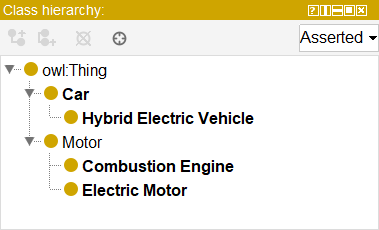
\includegraphics[width=0.9\linewidth]{fig/protege-asserted-class-hierarchy.png}
      \caption{Class hierarchy as asserted by the user}
      \label{fig:protege-asserted-class-hierarchy}
    \end{minipage}
    \begin{minipage}{.49\textwidth}
      \centering
      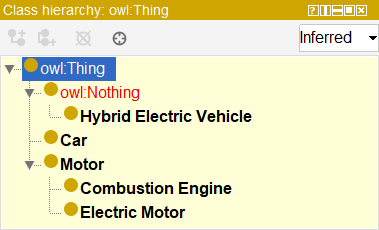
\includegraphics[width=0.9\linewidth]{fig/protege-inferred-class-hierarchy.png}
      \caption{Class hierarchy as inferred by the reasoner}
      \label{fig:protege-inferred-class-hierarchy}
    \end{minipage}
\end{figure}

\begin{example}
    In order for Alice to model the manufacturing process of cars, she includes the class \texttt{Motor} in her ontology as well as the subclasses \texttt{Electric Motor} and \texttt{Combustion Engine}, so she can describe the various parts of cars. She also decides to declare \texttt{Electric Motor} and \texttt{Combustion Engine} to be disjoint classes, as a motor can only be either electric or combustion.

    She also wants classes representing the final manufactured product. Therefore she decides to add the \texttt{Car} class to her ontology alongside the axiom \texttt{'Car' 'has part' exactly 1 'Motor'}.
    
    Later, as Alice decides to also include the various types of cars that are manifactured, she adds the class \texttt{Hybrid Electric Vehicle} as subclass of \texttt{Car}. She also adds the axiom \texttt{'Hybrid Electric Vehicle' 'has part' some 'Electric Motor' and 'Hybrid Electric Vehicle' 'has part' some 'Combustion Engine'}.

    After making her additions, Alice starts the reasoner in {\protege} and notices that it inferred \texttt{'Hybrid Electric Vehicle' EquivalentTo owl:Nothing} meaning that there can't be any hybrid electric vehicles. Due to the conflicting axioms of a \texttt{Car} having exactly 1 \texttt{Motor}, but the \texttt{Hybrid Electric Vehicle} being described as having two distinct types of motors, no individual can be an instance of \texttt{Hybrid Electric Vehicle}.
\end{example}

To use the reasoner in {\protege}, navigate to \textit{$\text{Reasoner}$}, select one like \textit{$\text{HermiT}$} and click on \textit{$\text{Start reasoner}$}.

The reasoner is only run if it is explicitly started by the user. If the ontology is changed, after the reasoner was run, the option \textit{$\text{Synchronize reasoner}$} in the tab becomes available, allowing the user to restart the reasoner for the updated ontology. It is therefore recommended to run the reasoner frequently during the development process.


% \subsubsection{Implementation in the Template Ontology}\label{sssec:implementation-in-the-mno}

% Identifiers look like this: MNO\_00010123

% They are structured in three parts: {[}Ontology{]}\_{[}yyyy{]}{[}xxxx{]}
% \begin{itemize}
%     \item ``{[}Ontology{]}\_'' identifies the ontology that this class belongs to. 
%     \item {[}yyyy{]} identifies the user who added the classes. Each user gets a unique ID.
%     \item {[}xxxx{]} identifies the
% specific class added by the user. 
% \end{itemize}

% This enables every user to create 10000 entities before having to get a new ID. IDs are assigned chronologically to each entity, starting with 0000.

